\chapter{Domain Driven Design}
\section{Analyse der Ubiquitous Language}
Das Programm wird im Rahmen einer Fahrgemeinschaft einer deutschsprachigen Gruppe von Informatikstudenten erstellt, weshalb Deutsch als Sprache für die Ubiquitous Language gewählt wird.

Die Beschreibung des Programms in \autoref{sec:funktionalität} entspricht dem Sprachgebrauch eines Domänenexperten, weshalb sich diese Wortwahl auch im Quellcode widerspiegeln sollte.
Die wichtigsten Begriffe sind hierbei:

\begin{itemize}
    \item Fahrgemeinschaft
    \item Fahrperiode
    \item Distanz (bestehend aus Betrag und Streckeneinheit)
    \item Fahrt
    \item Person (je nach Kontext auch als Mitfahrer bezeichnet, diese Begriffe sind austauschbar)
    \item Adresse (bestehend aus Straße und Ort)
    \item Telegram-Chat-ID
    \item PayPal-Link
\end{itemize}

Weiterhin wird festgelegt, dass für Informatikstudenten einzelne englische Begriffe keine Sprachbarriere darstellen, sondern vielmehr den alltäglichen Sprachgebrauch widerspiegeln.
Deshalb werden Getter- und Setter-Methoden weiterhin mit englischen Vorsilben konstruiert, um den Quellcode nah an Programmiersprachweiten Standards zu halten.

Aus der Funktionsbeschreibung des Programms und der Analyse der Ubiquitous Language ergibt sich das in \autoref{fig:domainmodel} dargestellte Domänenmodell.

\begin{figure}
    \centering
    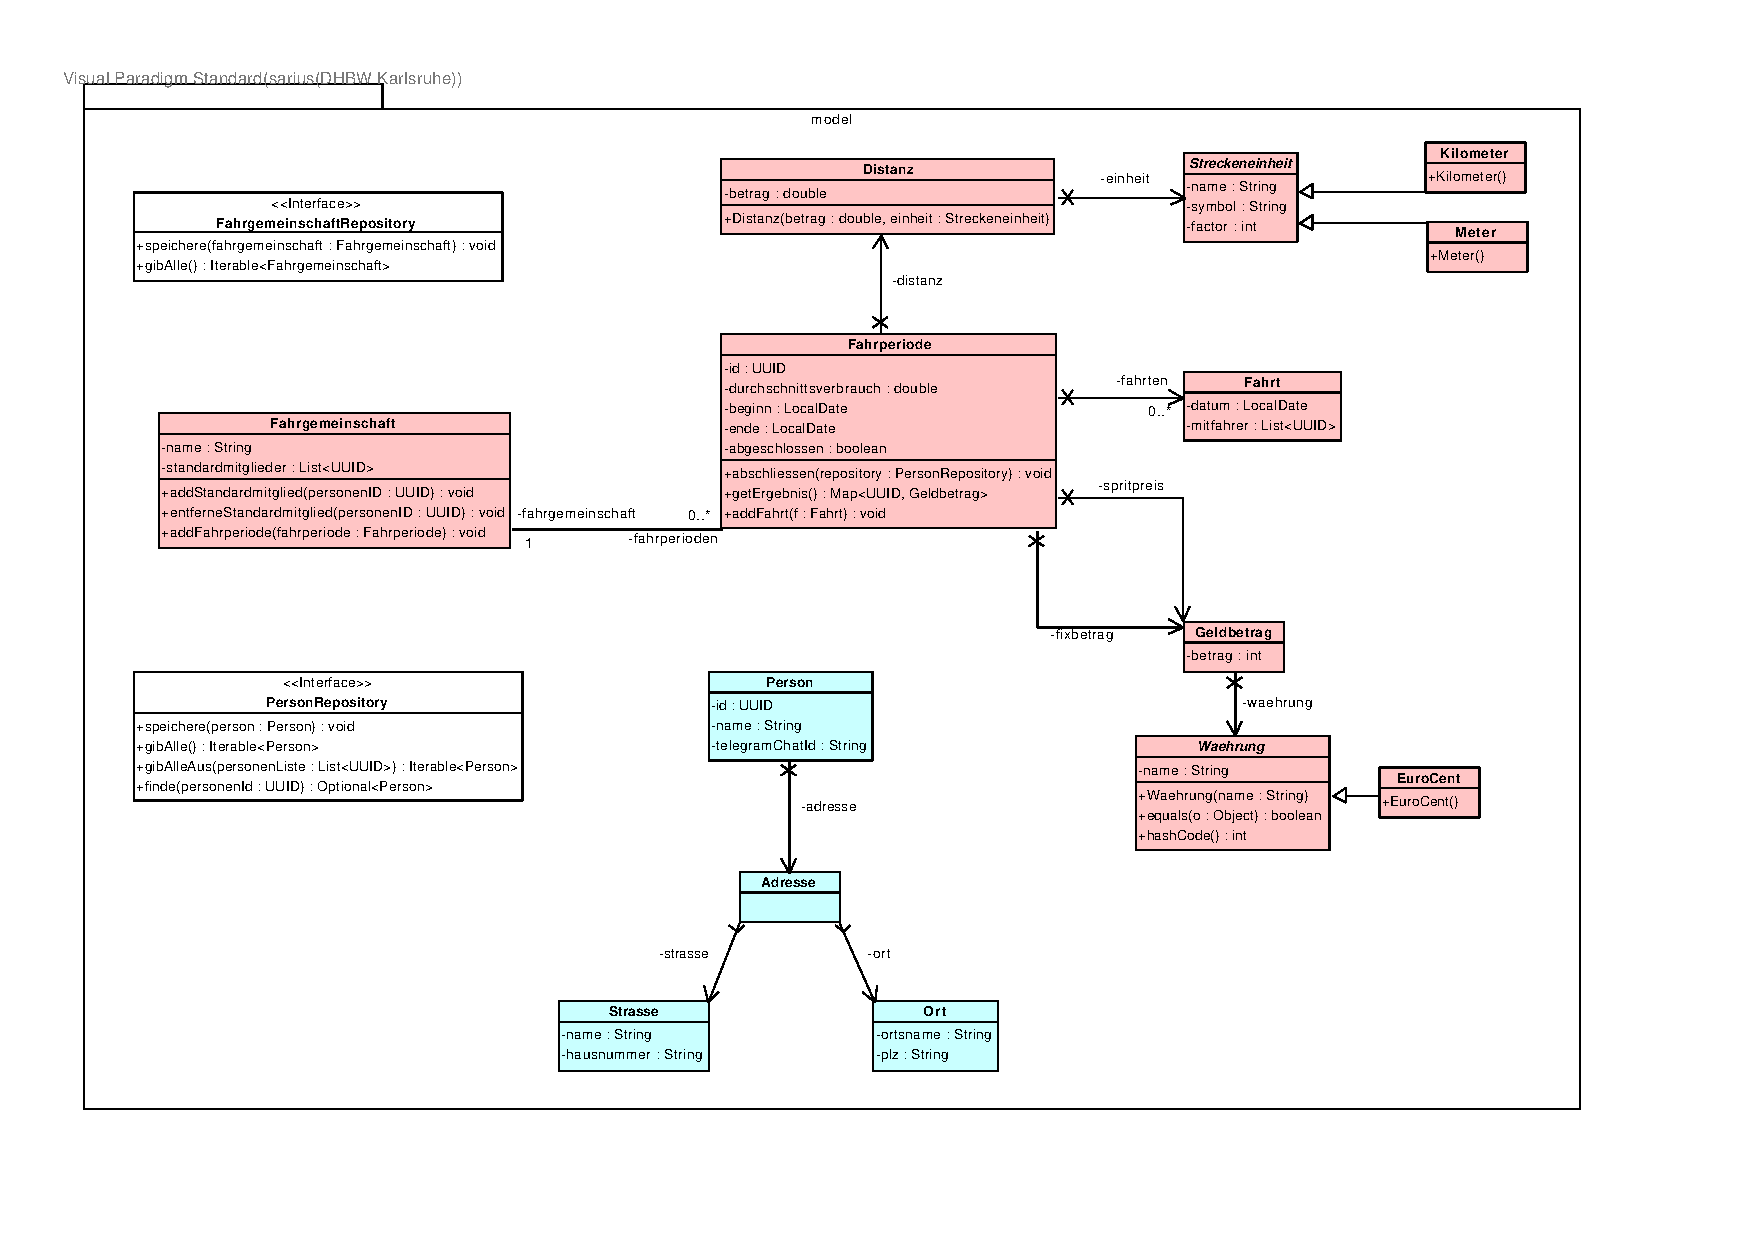
\includegraphics[width=1\textwidth, trim = 0cm 0cm 0cm 0cm]{../VPP/Domain Modell.pdf}
    \caption{Domänenmodell (\href{https://github.com/yschiebelhut/carpool-java/tree/27f64a9b6c1e387d7716d38462d01b4b0f8ff42a/3-carpool-java-domain/src/main/java/model}{Implementierung})}
    \label{fig:domainmodel}
\end{figure}

\section{Entities}
Im dargestellten Domänenmodell (\autoref{fig:domainmodel}) finden sich folgende Entitäten:

\begin{itemize}
    \item Person
    \item Fahrgemeinschaft
    \item Fahrperiode
\end{itemize}

Eine Person besitzt die Eigenschaften Name, Adresse und Telegram-Chat-ID, welche sich alle ändern können, ohne dass sich die Identität der Person ändert.
Einer Fahrgemeinschaft werden im Laufe der Zeit Fahrperioden und möglicherweise Mitglieder hinzugefügt, es ist jedoch weiterhin dieselbe Fahrgemeinschaft.
Ähnlich sieht es bei einer Fahrperiode aus, der nach und nach Fahrten hinzugefügt werden.
Hieran lässt sich ablesen, dass alle diese Klassen einen Lebenszyklus besitzen und somit als Entitäten einzuordnen sind.

Jede Entität verfügt über eine Identität.
Im Falle der Fahrgemeinschaft wird hierfür der Name der Fahrgemeinschaft als natürlicher Identifier gewählt, da ein Fahrer realistischerweise kaum mehr als eine Handvoll verschiedene Gruppen mitnimmt und es hier akzeptabel ist, einen Namen nur einmal vergeben zu können.
Für Person und Fahrperiode reichen die natürlichen Attribute nicht aus, um eine Entität eindeutig zu identifizieren.
Deshalb wird hier eine UUID als künstlicher Schlüssel vergeben.

\section{Value Objects}
Die restlichen, in \autoref{fig:domainmodel} dargestellten, Klassen werden als Value Objects realisiert.
Dies sind:

\begin{itemize}
    \item Distanz
    \item Unterklassen von Streckeneinheit
    \item Fahrt
    \item Geldbetrag
    \item Unterklassen von Waehrung
    \item Adresse
    \item Strasse
    \item Ort
\end{itemize}

Alle diese Klassen besitzen keinen Lebenszyklus und definieren sich rein über ihre Werte, weshalb sie auch keine Identität besitzen und sich somit nicht als Entität einordnen lassen.

\section{Aggregates}
Eine Adresse stellt eine Eigenschaft einer Person dar.
Weiterhin setzt sich eine Adresse aus einer Strasse und einem Ort zusammen.
Adresse, Strasse und Ort existieren nur im Kontext einer Person.
Wird die Person gelöscht, so existiert auch die zugehörige Adresse nicht mehr.
Deshalb werden Person, Adresse, Strasse und Ort zu einem Aggregat zusammengefasst.
Person ist in diesem Aggregat die einzige Entität und ist deshalb automatisch die Root-Entität.
Im Domänenmodell wird dieses Aggregat türkis hervorgehoben.

Im Falle von Fahrperioden stellen Distanz, Streckeneinheit, Fahrt, Geldbetrag und Waehrung Value Objects dar, die als Eigenschaften von Fahrperiode zu klassifizieren sind.
Deshalb werden diese Klassen zu einem Aggregat zusammengefasst.
Weiterhin existieren Fahrperioden jedoch nur im Kontext ihrer Fahrgemeinschaft.
Wird die Fahrgemeinschaft gelöscht, so entfernt dies auch die Fahrperioden.
Deshalb wird diesem Aggregat auch noch die Fahrgemeinschaft hinzugefügt und diese außerdem als Root-Entität gewählt.
Im Domänenmodell wird dieses Aggregat rot hervorgehoben.

\section{Repositories}
Gemäß dem Grundsatz \enquote{ein Repository pro Aggregat} werden zwei Repositories für den Zugriff auf den persistenten Speicher definiert.
Dies sind \emph{PersonRepository} und \emph{FahrgemeinschaftRepository}.
Diese erlauben jeweils den Zugriff auf die jeweilige Root-Entität des Repositories - also Person respektive Fahrgemeinschaft.
